\section{Microcanonical Ensemble}
\notedate{06/10/2022}
\gray{Recap: 
\begin{align*}
\text{Phase space} \qquad& \ps_N = \{(q_i,p_i) \qquad i = 1\dots N\}\\
\text{Hamiltonian} \qquad& \ham(q_i,p_i) : \ps_N \to \R
\end{align*}
}
The microcanonical ensemble represents a closed system that doesn't exchange either energy or matter with the environment, so in which the energy $E$, the number of particles $N$ and the volume $V$ are fixed. The evolution occurs on the hypersurface $S_E \subset \ps_N \qquad \ham (q_i,p_i) = E$\\

To describe the system we need the probability distribution of the microcanonical ensemble. We assume (a priori) a uniform probability:\\

\Def The probability distribution of the microcanonical ensemble is:
$$ \rho_{mc} (q_i,p_i) = C \delta (\ham(q_i,p_i) - E)$$
where $C$ is a constant we can obtain from the normalization:
$$ 1 = \int_{\ps_N} C\delta (\ham - E) = \int_{S_E} CdS_E = C\omega(E) \implies C = \frac 1{\omega(E)}$$
(reminding that $\omega(E)$ is the area of $S_\ham = E$). So:
\begin{equation} \label{eq:mcDist}
\rho_{mc} (q_i,p_i) = \frac 1{\omega(E)} \delta (\ham- E)
\end{equation}

Working with $S$ is difficult (e.g. it creates some problems when integrating), so we give an operative definition. We can write the volume of a phase space:
$$\Sigma(E) = \int_{0 \le \ham(q_i,p_i) \le E} d\Gamma = \int_0^E d\ham\omega(\ham)$$
from which,
$$ \Gamma(E) = \int _{E \le \ham \le E+\Delta E} d\Gamma = \int_E^{E+\Delta E} \omega(E') dE' = \stackrel{(if\ \Delta E\ small)}{\simeq}\omega(E)\Delta E $$

So we can see that the microcanonical probability density function (\ref{eq:mcDist}) is the limit for $\Delta E \to 0$ of:
$$ \rho_{mc} (q_i,p_i) = \begin{cases}
    \dfrac 1{\Gamma(E)} & E \le \ham \le E+\Delta E \\ 
    0 & \text{otherwise}
    \end{cases}
$$

\subsection{Microcanonical entropy \texorpdfstring{$S_{mc}$}{}}
\gray{We will see that it coincide with the thermodynamic entropy.}

$$ S_{mc} (E,V,N) \equiv k_B \log \omega(E)$$

\textbf{1)} We could actually define the entropy in three different ways:
\begin{enumerate}
    \item $S_{mc}^{(1)} = k_B \log \omega(E)$
    \item $S_{mc}^{(2)} = k_B \log \Gamma(E)$
    \item $S_{mc}^{(3)} = k_B \log \Sigma(E)$
\end{enumerate}
which in general are different quantities. However in the thermodynamic limit ($N,V \to \infty$, with $n= N/V const$), they represent the same quantity: 
$$s_{mc} = \frac{S_{mc}^{(1)}}N = \frac{S_{mc}^{(2)}}N = \frac{S_{mc}^{(3)}}N$$
\gray{So while doing calculations, we can use one of the three.}\\

\textbf{2)} Entropy should be extensive, so it should be additive: $ S_{mc}^A + S_{mc}^B = S_{mc}^{A\cup B}$\\

\Pf To prove it, let's call the phase space of the two systems: \\$\ps_1, \ps_2$. So $\ps_{AB} = \ps_1 \times \ps_2$

$$ d\Gamma_1 = \prod_{i=1}^{N_1} dq_idp_i \qquad d\Gamma_2 = \prod_{j=1}^{N_2} dq_idp_i \quad \implies \quad d\Gamma = d\Gamma_1 d\Gamma_2$$
If $\ham = \ham_1 + \ham_2 \implies E = E_1 + E_2 + E_{int}$.\\
Here we make an assumption: there could be interactions in the wall that divides the two systems, however, since $E_1$ and $E_2$ both scale with the volume ($L^3$) while $E_{int}$ scale like the area of interaction ($L^2$), we neglect the interaction term, because it disappears in the thermodynamic limit.

We can foliate the phase space with surfaces each at different energy


\begin{align*}
\omega (E) &= \int_{\ps_1 \times \ps_2} d\Gamma \delta(\ham - E)\\
&=\left(\int_0^\infty d\ham_1 \int dS_{\ham_1}\right) \left(\int_0^\infty d\ham_2 \int dS_{\ham_2}\right) \ \delta(\ham_1 + \ham_2 - E)\\
&= \int d\ham_1 \int d\ham_2 \delta(\ham_1 + \ham_2 - E) \int_{\ham_1=E_1} d s_{\ham_1} \int_{\ham_2 = E_2} dS_{\ham_2} \\
&= \int d\ham_1 \int d\ham_2 \delta (\ham_1+\ham_2 -E) \ \omega_1(E_1) \ \omega_2(E_2) \\
&= \int_0^E dE_1 \quad \omega_1(E_1) \ \omega_2(E_2=E-E_1)
\end{align*}

The integrand is $\ge 0$ and defined in a compact interval $[0,E)$, so it has a maximum. Let $E_1^*, E_2^* = E-E_1^*$ be the value of energy for which the integrand is maximum. So:

$$ \omega(E) \le \left(\int_0^E dE_1\right) \omega_1(E_1^*)\  \omega_2(E_2^*) \le E_1^* \ \omega_1(E_1^*) \ \omega_2(E_2^*)
$$
and for $\Delta E$ small enough:
$$ \Delta E\  \omega_1(E_1^*)\ \omega_2 (E_2^*) \le \Delta E \ \omega (E) \le E_1^* \ \omega_1(E_1^*) \ \omega_2(E_2^*) \ \Delta E
$$
Reminding that $\Gamma(E) \sim \omega(E)\Delta(E)$:

\begin{align*}
\Gamma_1(E_1^*)\Gamma_2(E_2^*) \le \Gamma(E) &\le \frac E{\Delta E} \Gamma_1 (E_1^*) \Gamma_2 (E_2^*) \\
\log\Gamma_1 + \log\Gamma_2 \le \log \Gamma &\le \log\Gamma_1 + \log \Gamma_2 + \log \frac E{\Delta E} \qquad (\times k_B) \\
S_{mc}^1 + S_{mc}^2 \le S_{mc} &\le S_{mc}^1 + S_{mc}^2 + k_B \log \frac E{\Delta E} \\
\end{align*}

In the thermodynamic limit, dividing everything by $N$ and letting $N\to \infty$, the last term approaches zero and can be neglected. So we find:
$$ S_{mc}(E) = S_{mc}^1(E_1^*) + S_{mc}^2(E_2^* = E-E_1^*)$$

\EndPf

\textbf{3)} In the thermodynamic limit, this entropy coincides with the thermodynamic entropy: $s_{mc} = s_{th}$ 

\Pf At equilibrium, $E = E_1^* + E_2^*$, where $\omega_1(E_1) \ \omega_2(E-E_1)$ is maximized.

\begin{align*}
    \Gamma(E_1^*) \Gamma(E_2^*) \to d\left.\left(\Gamma(E) = \Gamma_1(E_1) \Gamma_2(E_2)\right)\right|_{E_1 = E_1^*, E_2 = E_2^*} &= 0 \\
    \left.\left(\der{\Gamma_1}{E_1} dE_1\right) \Gamma_2 + \Gamma_1 \left(\der{\Gamma_2}{E_2} dE_2\right)\right|_{E_1^*, E_2^*} &= 0 \\
    \gray{(dE_2 \to dE_1)} \qquad \frac{\Gamma_1}{\Gamma_1\Gamma_2}\left(\left.\der{\Gamma_1}{E_1} \Gamma_2 \right|_{E_1^*, E_2^*} = \left.\Gamma_1\der{\Gamma_2}{E_2}\right|_{E_1^*, E_2^*}\right)
\end{align*}
\begin{align*}
    \left.\frac 1{\Gamma_1} \der{\Gamma_1}{E_1}\right|_{E_1^*} &= \left.\frac 1{\Gamma_2} \der{\Gamma_2}{E_2}\right|_{E_2^*} \\
    \left.\der{}{E_1} k_B\log\Gamma_1(E_1)\right|_{E_1^*} &= \left.\der{}{E_2} k_B\log\Gamma_2(E_2)\right|_{E_2^*} \\
    \left.\der{}{E_1} S_{mc}^1\right|_{E_1^*} &= \left.\der{}{E_2} S_{mc}^2\right|_{E_2^*} \\
\end{align*}
\gray{since this is calculated at $E_1^*, E_2^*$, it is calculated at the equilibrium ($N,V$ fixed).}

The same thing happens in thermodynamic: if $T_1=T_2$, 
$$dE = TdS_{th} - pdV+ \mu dN \implies \frac 1T = \left.\der{S_{th}}E\right|_{V,N}$$
So the equilibrium in thermodynamics requires this condition:
$$\boxed{\der{S_{th}^1}{E_1} = \der{S_{th}^2}{E_2}}$$

So we find that: 
$$ S_{th}(E,V,N) = S_{mc}(E,V,N) = k_B\log\Gamma(E)$$
(equal and not only proportional, because $k_B$ is the constant appositely chosen to make them equal)

\EndPf

\textbf{4)} We saw that 
$$\angles f_{mc} = \int_ {\ps_N}\left(\prod dp_i dq_i\right) f(q_i,p_i) \rho_{mc}(q_i,p_i) $$
We can now prove the Universal Boltzmann's formula (works in the TD-limit):
$$ S_mc = -k_B \angles{\log\rho_mc}_{mc}$$

\Pf Working from the Universal Boltzmann's formula, we can arrive to the definition of entropy

\begin{align*}
    -k_B \angles{\log\rho_mc}_{mc} &= -k_B\int_{\ps_N} d\Gamma(\log\rho_{mc})\rho_{mc} \qquad \gray{\rho_{mc} = \frac 1{\omega(E)} \delta(\ham-E) \implies \rho_{mc}|_{S_c} = \frac 1{\omega(E)}} \\
    &= -k_B\int_{S_E} \frac 1{\omega(E)}(-\log \omega(E)) \\
    &= k_B \frac 1{\omega(E)} \log \omega(E) \int_S dS_E \\
    &= k_B \log \omega (E) = S_{mc}
\end{align*}

So we have proved that, in the TD-limit:
$$ S_{mc} = k_B \log \Sigma = k_B\log\Gamma = k_B\log \omega = -k_B\angles{\log\rho_{mc}}_{mc}$$

\subsection{One example/exercise (1.1, 1.2): Perfect gas}
We consider a gas of $N$ non-relativistic and non-interacting monoatomic particles in 3D, confined in a volume $V$.
$$
 \ps_N = \{\{(\vec q_i, \vec p_i)\}_{i=1}^N : \vec q_i \in V, \vec p_i \in \R^3 \} \qquad 
 \ham(q_i,p_i) = \sum_{i=1}^N \frac{\vec p^2_i}{2m}
$$
The volume of states is:
$$ \Sigma(E) = \int \prod_{i=1}^N \frac{d^3q_i d^3p_i}{h^3}$$
where the integral is calculated on:
$$ 0 \le \ham(q_i, p_i)\le E \qquad 0 \le \sum_{i=1}^N {\vec p_i}^2 \le 2mE \qquad 0 \le \sum_{i=1}^N\left({p_i^{(x)}}^2+ {p_i^{(y)}}^2 + {p_i^{(z)}}^2\right) \le 2mE$$
So it is the volume of a $3N$-dimensional sphere of radius $\sqrt{2mE}$. So:
\begin{align*}
\Sigma(E) &= \frac 1{h^{3N}}\left(\int_V d^3 q_i\right)^N \int_{0 \le \sum \vec p_i^2 \le 2mE} \prod_i \vec p_i^2 \\
&= \frac{V^N}{h^{3N}}\Omega_{3N}(R= \sqrt{2mE}) \\
&= \frac{V^N}{h^{3N}} \frac{2\pi^{3N/2}}{(3N)\Gamma(3N/2)}(R=\sqrt{2mE})^{3N}
\end{align*} 
where $\Gamma(x) = \int_0^\infty dt\ t^{x-1}e^{-t}$ is the Euler's $\Gamma$-function, which can be seen as a generalization of the factorial. \gray{In fact, one can prove (integrating by parts) that\\ $\Gamma(n) = (n-1)! \qquad \Gamma(x+1) = x\Gamma(x) \qquad \log\Gamma(x) \simeq x\log x - x$}\\

The previous formula is composed by an angular part (the Euler's $\Gamma$-function) and a radial part (which scale with $3N$). So finally we have that:
$$ \Sigma(E) = \frac 23 \left(\frac{V}{h^3}\right)^N \frac {(2\pi mE)^{3N/2}}{N\Gamma (3N/2)} $$

Calculating the derivative, one can also get the density of the states and $d\Gamma$:
$$ \omega(E) = \der\Sigma E = \frac {3N}{2E} \Sigma(E) \qquad \Gamma(E) = \omega(E)\Delta E = \frac{3N}{2E} \Sigma(E) \Delta E$$

and we can check that in the TD-limit, the different ways of defining the entropy are the same:
$$\frac{\log \Gamma}N = \frac{\log \omega}N + \cancel{\frac{\log \Delta E}N} = \frac{\log \Sigma}N + \cancel{\frac{\log \Delta E}N} + \cancel{\frac{\log \frac{3N}{2E}}N}$$
where the terms can be cancelled in the limit of $N\to \infty$ (for the last one, since $E \sim N$, the ratio $3N/2E$ is constant).\\

We can then find the entropy for a perfect gas (supposing distinguishable particle)
\begin{align*}
    S_{dis} &= k_B \log \Sigma(E) \\
    &= k_B\left[N\log\left(V\left(\frac{2\pi mE}{h^2}\right)^{3/2}\right) - \cancel{\log N} - \log \Gamma\left(\frac{3N}2\right) + \cancel{\log\frac23}\right] \quad &(TD-limit)\\
    &= k_B\left[N \log\left(V\left(\frac{2\pi mE}{h^2}\right)^{3/2}\right) - \frac{3N}2 \log\frac{3N}2 + \frac{3N}2\right] \quad &(Stirling) \\
    &= k_B\left[\frac{3N}2 + N\log\left(V\left(\frac{4\pi mE}{3Nh^2}\right)^{3/2}\right)\right]\\
\end{align*}

\notedate{(III) MON 10/10/2022}
This formula has a problem: it is not extensive: if $N \to 2N$ and $V \to 2V$ we expect $S \to 2S$, but we actually have $S \to 2S + N\log 2$.

The solution is to consider indistinguishable particles. That means that the states: 
$\qquad  (q_1,p_1, q_2, p_2, \dots, q_n,p_n) \qquad (q_2,p_2, q_1, p_1, \dots, q_n,p_n)  $ \\
which are different points in the phase space $\ps_N$, should be counted only once. We have $N!$ of this equivalent vectors, so $\Sigma (E) \to \Sigma(E) / N!$, and we get:

\begin{align} \label{eq:entropy-indistinguishable}
S_{ind} &= k_B\log\frac{\Sigma(E)}{N!} \nonumber \\
&= k_B \left[\log\Sigma(E) - \log N!\right] \nonumber \\
&= k_B \left[\frac52 N + N\log \left(\frac VN \left(\frac{4\pi m E}{3Nh^2}\right)^{3/2}\right)\right] 
\end{align}

which is an extensive quantity.

So for an ideal gas in 3D microcanonical we have:
\begin{align*}
 d\Omega &= \prod_{i=1}^N \frac{d^dq_id^dp_i}{h^d} &\qquad \text{distinguishable particles} \\
 d\Omega &= \frac1{N!}\prod_{i=1}^N \frac{d^dq_id^dp_i}{h^d} &\qquad \text{indistinguishable particles}
\end{align*}

From the entropy, knowing that $TdS = dE + pdV - \mu dN $, we can get:
\begin{itemize}
    \item $$\frac 1T = \left.\der SE\right|_{V,N} = [\dots] = \frac 32 \frac{Nk_B}E$$     \begin{equation} \label{eq:thermal-energy}
        \boxed{ E = \frac32 Nk_B T} \qquad \text{Thermal energy of an ideal gas}
    \end{equation}
    (where the 3 stands for the number of dimension)
    \item $$\frac pT = \left.\der SV\right|_{E,N} = \frac {Nk_B}V \implies \boxed{pV = k_BNT}$$
    \item $$ \frac \mu T = \left.\der SN\right|_{E,V} \implies \mu = \dots$$ 
\end{itemize}

Substituting \ref{eq:thermal-energy} in \ref{eq:entropy-indistinguishable} we get:
$$ S = \frac 52 Nk_B + k_B N\log \left[\frac VN\left(\frac{2\pi m k_B T}{h^2}\right)^{3/2}\right] = \frac 52 N k_B + 3 Nk_B \log \left(\frac d{\lambda_T}\right)$$
where we have defined the \textit{thermal wavelength} $\lambda_T$ and the average inter-particle distance $d$ as:
$$ \lambda_T \equiv \sqrt{\frac{h^2}{2\pi m k_BT}} \qquad v = \frac VN = \frac 1n \simeq d^3$$

\gray{These formulas have a problem: it might happen that for low temperature $T, d \underset\sim< \lambda_T, S < 0$ !. So something break down when $d \sim \lambda_T$, but there will be a quantum mechanical solution. However, what we have found is true until $d > \lambda_T$, otherwise we have interaction effects.}

\section{Canonical Ensemble}
\begin{align*}
    \text{System} \qquad & \syst = \{(q_i^{(1)}, p_i^{(1)})\},\quad  V_1 \ll V_2, \quad N_1 \ll N_2 \\
    \text{Environment} \qquad & \varepsilon = \{(q_i^{(2)}, p_i^{(2})\}, \quad V_2, N_2
\end{align*}
We have a system and an environment with a wall in between them that permits heat and energy to pass but not particles. Energy is exchanged, but the total energy $E \equiv E_1 + E_2 = const.$ (with $E_1 \ll E$), so that the universe $\U = \syst \cup \varepsilon$ is microcanonical.

The phase space is $\ps_\U = \ps_1 \times \ps_2$ and:
$$ d\Omega_\U = d\Omega_1 d\Omega_2 \propto \left(\prod_{i=1}^{N_1} dq_i^{(1)}dp_i^{(1)}\right)\left(\prod_{j=1}^{N_2} dq_j^{(2)}dp_j^{(2)}\right)$$
$$ \rho_{mc}\left(q_i^{(1)}, p_i^{(1)};q_j^{(2)},p_j^{(2)}\right) = \frac{\delta(\ham_1 + \ham_2 - E)}{\omega(E)}$$

The whole universe is described with a microcanonical probability distribution function, and the (canonical) probability distribution describing the system only is obtained by integrating out the environment d.o.f. So:
\begin{align*}
 \rho_c^{(\syst)}\left(q_i^{(1)},p_i^{(1)}\right) &\propto \int \rho_{mc}(\ ) d\Omega_2 \qquad \delta\text{ is selecting only the surface with $E_2 = E-E_1$} \\
 &= \frac 1{\omega(E)} \int_{E_2=E-E_1}d\Omega_2 \\
 &= \frac{\omega(E_2 = E-E_1)}{\omega(E)}
\end{align*}
So $\rho_c^{(\syst)}\left(q_i^{(1)},p_i^{(1)}\right) \sim \omega_2(E_2 = E-E_1)$ and we know that $S = k_B \log \omega$, so:
\begin{align*}
\log \rho_c \sim \log \omega_2(E_2) &\sim S_2(E_2=E-E_1) \\
(E_1 \ll E) \qquad &\simeq S_2(E) + \left.\der{S_2}{E_2}\right|_{E_2=E} (-E_1) + \dots \\
&= S_2(E) - \frac{E_1}{T_2(=T_1=T)}
\end{align*}

$$\implies \log \rho_c \sim \log \omega_2 \sim \frac 1{k_B} \left(S(E) - \frac{E_1}T\right)$$
$$ \implies \rho_c \left(q_i^{(1)}, p_i^{(1)}\right) = e^{S_2(E)/k_B} \ e^{-E_1/k_B T} \simeq e^{-E_1/k_B T} $$since the first term is a constant.

We can see that it depends only on the system $(E_1)$. Defining $\beta = 1/k_BT$:
$$ \rho_c \left(q_i^{(1)}, p_i^{(1)}\right) = (const) \ e^{-\beta \ham\left(q_i^{(1)}, p_i^{(1)}\right)}$$

We have eliminated the environment, so we will avoid writing the subscript $^{(1)}$ from now on:
$$ \rho_c (q_i,p_i) = \frac 1{Z_N} e^{-\beta\ham(q_i,p_i)}$$
where he have defined the \textbf{canonical partition function} $Z_N$, which can be determined with the normalization:
$$ 1 = \int_{\ps_1} \rho_c d\Omega = \frac1{Z_N} \int_{\ps_\syst} \prod_{i=1}^N \left(\frac{dq_idp_i}{h^d}\right) e^{-\beta\ham(q_i,p_i)}$$
$$ \implies Z_N \equiv \int_{\ps_\syst} \left(\prod_{i=i}^N\frac{dq_idp_i}{h^d}\right) e^{-\beta\ham(q_i,p_i)}$$
\gray{$Z_N = Z_N(T,V)$ depends on $N,T,V$.}\\

This expression is valid for distinguishable particles. For indistinguishable particles there is a $1/N!$ factor. For simplicity we write:
$$ d\Omega = \frac 1{\xi_N} \prod_{i=1}^N \frac{dq_idp_i}{h^d} \qquad \text{with }\xi_N = \begin{cases}
    1 & \text{distinguishable} \\
    N! & \text{indistinguishable}
\end{cases}$$

Using the fact that we can foliate the phase space, we can write \gray{(assuming the lowest bound to be 0)}:
$$ Z_N(V,T) = \int_\ps d\Omega e^{-\beta\ham} = \int_0^\infty dE \int_{S_\ham=E} dS_\ham e ^{-\beta\ham} = \int_0^\infty dE \ \omega(E) e^{-\beta E}$$

\gray{In systems with a discrete set of energies values $E_j$: $Z_N = \sum_j e^{-\beta\epsilon_j} g_j$}\\

\textbf{1)} For more species $A,B, \dots$ of particles, we can assume that there is no interaction among different species: $ \ham = \ham_A + \ham_B$. So:
\begin{align*}
Z_N &= \int d\Omega_A d\Omega_B \dots \ e^{-\beta(\ham_A+ \ham_B + \dots)} \\
&= \left(\int d\Omega_A e^{-\beta\ham_A}\right)\left(\int d\Omega_B e^{-\beta\ham_B}\right)\dots \\
&= Z_{N_A}^A Z_{N_B}^B \dots
\end{align*}
So if the species are distinguishable and independent one from the others (not interacting), the partition function is the product of the partition function of all the species.\\

\textbf{2)} Given an observable $f(q_i,p_i)$, the canonical average is:
$$ \angles f_c \equiv \int_\syst d\Omega \rho_c(q_i,p_i) f(q_i,p_i) = \frac 1{Z_N} \int_\syst d\Omega e^{-\beta \ham(q_i,p_i)} f(q_i,p_i)$$

\subsection{Thermodynamic quantities}
We recover the thermodynamic potentials, by defining:\\

\textbf{1)} $$F(T,V,N) = -\frac 1\beta \log Z_N(T,V) \qquad (\iff Z_N = e^{-\beta F})$$

\textbf{2)} $$E = \angles\ham_c = -\der{\log Z_N}{\beta}$$

\Pf We can see that both $Z_N$ (microscopic description) and $F$ (macroscopic) depend on $N,V,T$. This leads us to think that it must be related,  We will see that: $Z_N = e^{-\beta F} \quad F = -\frac 1{\beta} \log Z$
$$ e^{-\beta F} = Z_N = \int d\Omega e^{-\beta\ham} \implies \int d\Omega e^{-\beta (\ham-F)} = 1$$
Differentiating both sizes $\left(\der{}\beta\right)$ : 
$$ \int d\Omega e^{-\beta(\ham-F)} \left[F-\ham + \beta \der F\beta\right] = 0$$

\gray{As an exercise, since  $\beta = \frac1{k_BT} \qquad \beta \der{}\beta = -T\der{}T $}

$$ \implies F = \frac{\int d\Omega \ham e^{-\beta \ham}}{e^{-\beta F} = Z_N} + T \left.\der FT\right|_{V,N} = \angles \ham_c + T\der FT$$

While in thermodynamic we have $F_{th} = E_{th} - TS \qquad S = -\left.\der {F_{th}}T\right|_{V,N}$.\\
These two expressions are the same if we identify: 
$$F_{th} = F = -\frac1\beta \log{Z_N} \qquad S_{th} = -\left.\der FT\right|_{V,N} \qquad E = \angles \ham_c = \frac{\int d\Omega \ham e^{-\beta \ham}}{\int d\Omega e^{-\beta\ham}}$$

\EndPf

\gray{A useful formula in exercises:
$$ E = \angles \ham_c = \frac 1{\int e^{-\beta\ham} = Z_N} \der{}\beta \left(\int e^{-\beta\ham}\right) = - \der {}\beta \log Z_N$$}\\

\textbf{3)} We saw the universal Boltzmann's formula in the microcanonical. In the canonical it is the same (that's why it's called \textit{universal}):
$$ \boxed{S = -k_B \angles{\log \rho_c}_c}$$

\Pf 
\begin{align*}
    -k_B\angles{\log \rho_c}_c &= -k_B\int d\Omega \rho_c \log \rho_c \\
    &= -kB \int d\Omega \frac{e^{-\beta \ham}}Z (-\beta\ham - \log Z) \\
    &= k_B\left[\beta \int d\Omega \frac{e{-\beta\ham}}Z\ham + \log Z \frac{\int d\Omega e^{-\beta \ham} = Z}Z\right] \\
    &= k_B\left[\frac 1{k_BT}\angles\ham_c + \log Z\right] \qquad \left(F = -\frac 1\beta \log Z \implies \log Z = \frac 1{k_BT}F\right) \\
    &= \frac {E-F}T = S
\end{align*}

\subsection{Equipartition theorem}
\Th Let $\xi_1 \in [a,b]$ denote one of the canonical coordinates $(q)$ or momenta $(p)$ and $\xi_j \ ; \ (j\ne 1)$ all other variables. Suppose that the following condition holds:
$$ \int\left(\prod_{j\ne1} d\xi_j\right) \left[\xi_1 e^{-\beta \ham}\right]_a^b = 0$$

Then:
$$ \angles{\xi_1\der\ham{\xi_1}}_c = k_BT$$

\Pf 
$$1 = \int d\Omega \rho_c = \int d\xi_1\left(\prod_j d \xi_j\right) \frac{e^{-\beta\ham}}Z $$
But we can write the differential $d_{\xi_1} = \frac d{d\xi_1} \partial\xi_1$ :
$$ d\xi_1 e^{-\beta\ham(\xi_1,\xi_j)} = d_{\xi_1} \left( \xi_1 e^{-\beta\ham}\right) - \xi_1(-\beta) e^{-\beta\ham} \der \ham{\xi_1} d\xi_1$$
So we obtain:
\begin{align*}
    1 = \int\left(\prod_{j\ne 1} d\xi_j\right) d_{\xi_1} \left[\xi_1 \frac{e^{-\beta\ham}}Z\right] + \int \left(d\xi_1 \prod_{j\ne1} d\xi_j\right) \frac 1{k_BT} \frac{e^{-\beta\ham}}Z \der \ham{\xi_1} \xi_1
\end{align*}
And from the hypothesis, the first term is zero. So:
$$ k_BT = \int d\Omega \rho_c\left(\xi_1\der\ham{\xi_1}\right) = \angles{\xi_1\der\ham{\xi_1}}_c$$
$$ \implies \angles{\xi_1\der\ham{\xi_1}}_c = k_BT $$

\EndPf

We can now see that the standard equipartition theorem is a corollary of this: \\
If the coordinate $\xi_1$ appears quadratically in the Hamiltonian, then it contributes to the internal energy with an addend of $k_BT/2$.

Indeed, if: $\ham = A\xi_1^2 + \tilde \ham (\xi_j)$ :
$$\xi_1\der\ham{\xi_1} = 2A\xi_1^2 = 2\ham_1 \implies 2 \angles{\ham_1}_c = k_BT \implies \angles {\ham_1}_c = \frac{k_BT}2$$

Let's analyze better the condition of the theorem:
$$ \xi_1 \in [a,b] \qquad \left[\xi_1 e^{-\beta\ham(\xi_1,\xi_j)}\right]_a^b = 0$$
\begin{wrapfigure}{r}{0.3\textwidth}
    \centering
    %\resizebox{4cm}{!}{
    \begin{tikzpicture}
        \draw[->](0,2) -- (5,2) node[anchor=west] {$q$};
        \draw(0.5,4) -- (0.5,0) node[anchor=west] {$a$};
        \draw(4.5,4) -- (4.5,0) node[anchor=east] {$b$};
        \draw(2.5,0) parabola (4.25,4);
        \draw(2.5,0) parabola (0.75,4);
    \end{tikzpicture}
    %}
\end{wrapfigure}

\begin{itemize}
    \item Suppose $\xi_1 = q$, then: $\ham = \ham_{KIN} + V(q)$. The requirement becomes:
    $$q \in [a,b] \qquad \left.e^{-\beta V(q)}\right|_a^b = 0 \implies V(q\to a,b) = \infty$$
    which is not a strange condition in physics, where usually the particle is confined.
    \item Suppose $\xi_1 = p$, then: $\ham _{KIN} = \frac{p^2}{2m}$ and the requirements becomes:
    $$ p \in [-\infty,+\infty] \qquad \left[e^{-\beta\frac{p^2}{2m}}\right]_{-\infty}^{+\infty}$$
    There are some magnetic systems which don't satisfy this condition, but in general it is satisfied.
\end{itemize}

\subsection{Exercise (2.1): Find the partition function of a (classical) perfect gas in 3D}
$$ \ps_N = V^N \times \R^{3N} \qquad \vec{q} \in V \quad \vec p \in \R^3 \qquad \ham(q_i,p_i) = \sum_{i=1}^N \frac{{\vec p_i}^2}{2m}$$
$$ \rho_c(q_i,p_i) = \frac{e^{-\beta\ham}}{Z_N}$$
\begin{align*}
Z_N &= \frac1{N!\left(h^3\right)^N} \int_V \prod_{i=1}^N d^3q_i \int_{\R^3}\left(\prod_{i=1}^N d^3 p_i\right) e^{-\beta \sum_{i=1}^N \frac{\vec p_i^2}{2m}}\\
&= \frac{V^N}{N!h^{3N}} \left(\int_{\R^3} d^3p e ^{-\beta \frac{\vec p^2}{2m}}\right)^N \qquad \qquad (p^2 = p_x^2 + p_y^2 + p_z^2) \\
&= \frac{V^N}{N!h^{3N}} \left(\int_{-\infty}^{+\infty} dp_\alpha e ^{-\beta \frac{p_\alpha^2}{2m}}\right)^{3N} \qquad \qquad \text{Gaussian integral}
\end{align*}
$$ \boxed{Z_N = \frac{V^N}{N!}\left(\frac{\sqrt{2mk_BT}}h\right)^{3N} = \frac{V^N}{N!} \frac 1{\lambda_T^{3N}} }$$

Generalizing in d-dimension: $Z_N = \dfrac{V^N}{N!} \dfrac1{\lambda_T^{dN}}$\\

From that partition function we can get:
\begin{itemize}
    \item $$ E = -\der{}\beta \log Z_N = \frac 32 N k_BT $$
    which agrees with the equipartition theorem: $\ham = \frac12 (p_x^2 + p_y^2 + p_z^2)$: \\3 quadratic variables $\implies 3\frac{k_BT}2$
    \item 
    \begin{align*}
    F &= -\frac 1\beta \log Z_N = -k_BT \left[N\log V{\lambda_T^3} - \log N!\right] \qquad (Stirling)\\
    &= k_BT N\left[\log \frac{\lambda_TN}V - 1\right]
    \end{align*}
    $$ \frac FN = f = k_BT\left(\log \frac{\lambda_T N}V - 1\right)$$

    \item $S = \frac{E-F}T$ (as an exercise) or:
    $$ S = -\left.\der F T\right|_{V_N} = k_B N\left[\frac52 - \log (n\lambda_T^3)\right] $$
    \gray{Notice that in both cases the result is the same and implies $S=0$, for $T< \frac{n^{2/3}h^2}{2\pi m k_B e^{5/3}}$. This is of course absurd, signalling that this model is not suited to describe the low temperature limit.}
    \item $$ p = -\left.\der F V\right|_{T,V} = \frac{k_BT N}V \iff pV = Nk_BT$$
\end{itemize}

\notedate{13/10/2022}
\begin{wrapfigure}{r}{0.3\textwidth}
    \centering
    %\resizebox{4cm}{!}{
    \begin{tikzpicture}
        \draw[->](0,1.5) -- (5,1.5) node[anchor=west] {$T$};
        \draw[->](0.5,0) -- (0.5,3.5) node[anchor=east] {$\beta\mu$};
        \draw(0.75,3.5) .. controls(1,1.5) and (2,0.5) .. (5,0.5);
    \end{tikzpicture}
    %}
\end{wrapfigure}

\begin{itemize}
    \item $$ \boxed{\mu = \left. \der FN\right|_{T,V} = k_BT \log n\lambda_T^3}$$
    Relation between $\mu\lrarr n$ at fixed $T$
    
    Or, choosing the density: $\mu = \mu(T)$ (in graph). We can see that: $\mu(T) \xrightarrow[T\to\infty]{}\infty$ \qquad and \qquad $\boxed{\der\mu T < 0}$ 
    
    \gray{This condition will play an important role in a Bose-Einstein gas}
\end{itemize}

\begin{itemize}
    \item Specific heat: 
    $$\C_V = T \left.\der ST\right|_{V,N} = \left.\der ET\right|_{V,N} = \frac 32 NK_B \qquad c_V = \frac {\C_V}N = \frac 32k_B \qquad \text{Dulong-Petit law}$$
    $$\C_p = T \left.\der ST\right|_{p,N} = \left.\der ET\right|_{p,N} + p\left.\der VT\right|_{p,N} = \frac 32 NK_B + Nk_B = \frac52k_BN \qquad c_p = \frac {\C_p}N = \frac 52k_B$$
\end{itemize}
\gray{Notice that $c_V$ comes out to be constant: this is in contradiction with thermodynamic identities that require $cV \to 0$ as $T \to 0$. Again this shows that this model is not suited to describe the low temperature limit.}

\subsection{Magnetic systems}
Another way to make work is through magnetic interaction.\\ So: $dE = \delta Q -\delta\work + \mu dN = TdS - pdV + dE_{mag}$

If $\vec E, \vecP$ are the external field and the reaction of the matter to the external field respectively, we can define $\vec D$ as the Total magnetic field: $\vec D = \epsilon_0 \vec E + \vecP$\\
\gray{For historical reasons, $\vecP$ contains in its definition the factor $\epsilon_0$ already.}

The Maxwell equations in matter becomes:
$$ \nabla \cdot \vec D = \rho \qquad \nabla \cdot \vec B = 0 \qquad \nabla \times \vec E = -\der {\vec B}t \qquad \nabla \times \vec H = \vec j + \der {\vec D}t$$
where: $\vec H = \vec B / \mu_0 - \vec \ps$

A charged particle is described by $\vec F_{el} = q\vec E \qquad \vec E = \vec \nabla V$
And we have:
$$\ham_0 = \frac{\vec p^2}{2m} + QV(q)$$
where $V(q)$ is the elastic potential energy.\\

There could be some other effects, like some atoms or molecules could have a dipole moment $\vec d$ (e.g. water molecule). This dipole can be seen by an external field, because of the interaction $\vec d \cdot \vec E$. However this effect is usually not very strong ($\vecP$ is weak), with the exception of the ferromagnetic materials.

We have different materials with different effects: diamagnetism, paramagnetism, ferromagnetism.\\

\textbf{Paramagnetism} The assumptions for paramagnetism are that:
\begin{itemize}
    \item There are no macroscopic charge or net current flow
    \item As we said, $\vecP$ is negligible with respect to magnetisation.
    \item We assume $\rho =0$, from which the Maxwell equations become:
\end{itemize}
$$ \vec \nabla \cdot \vec D = \epsilon_0 \vec \nabla \cdot \vec E = 0 \qquad 
\vec \nabla \cdot \vec B = 0 \qquad
\vec \nabla \times \vec E = -\der{\vec B}t \qquad
\vec \nabla \times \vec H = \vec j $$

We can define the total magnetization (an extensive quantity) as:
$$ \vec M = \int_V d^3 q \vec \ps(q) = V\vec \ps$$
And we have: $\vec B = \mu_0 \vec H + \mu_0 \vec \ps(q)$, so:

\begin{align*}
\delta \work  &= dt \int_V d^3 q \vec j \cdot \vec E \\
&= dt \int_V d^3 q \left(\vec \nabla \times \vec H\right) \cdot \vec E \\
&= dt \int_V d^3q\left[\vec \nabla \cdot \left(\vec H \times \vec E\right) + \vec H \cdot \left(\vec \nabla \times \vec E\right)\right] \\
&= dt \left[\vec H \times \vec E\right]_{\partial V} + dt \int_V d^3 q \vec H + \der {\vec B}t \qquad \text{the first is a boundary term}\\
&= \int_V d^3 q \vec H \cdot \left(d \vec B\right) = d E_{mag} \\
&= \mu_0 \int_V d^3 q \vec H \cdot d\left(\vec H + \vec \ps\right)
\end{align*}
If we suppose an homogeneous material, $\vec H$ is uniform, so $\vec \ps $ is uniform too. We obtain:
$$ \delta \work = \mu_0 V \vec H \cdot d \vec G + \mu_0 V \vec H \cdot d\vec \ps 
= V\mu_0 d \left(\frac{H^2}2\right) + \mu_0 \vec H \cdot d\vec M$$
The first term is not relevant, since it's the same we have in vacuum.

The total energy can thus change for more reasons:
$$ d\vec  E = TdS - pdV + \mu dH + \mu_0 \vec H \cdot d\vec M$$
and $\vec H, \vec M$ are a couple of conjugated variables, just like $(T,S), (p,V), (\mu,N)$.

If we apply this to a solid ($dV = 0$) in the canonical ensemble ($dN = 0$):
\begin{itemize}
    \item internal energy: $ dE = TdS + \mu_0 \vec H \cdot d\vec M \implies E = E(S,\vec M)$\\
    from which: $T = \left.\der ES\right|_M \qquad \vec H = \left.\der E{\vec M}\right|_S$ \quad (not so useful)
    \item Helmotz free energy: $F = E-TS \qquad dF = SdT + \mu_0 \vec H \cdot d\vec M$
    \item Gibbs free energy: $G = E-TS - \mu_0 \vec H \cdot \vec M \qquad dG = -SdT - \mu_0 \vec M \cdot d\vec H$\\
    from which: $\vec M = \left.\der G{\vec H}\right|_T$ \quad (more useful, since we want the internal $\vec M$, given the external magnetisation $\vec H$)
\end{itemize}

\gray{Microscopically, paramagnetism is correlated to dipole molecules: the intrinsic magnetic moments $\vec \mu$ (which is due to electrons orbiting around nuclei (microscopical current) or due to spin) can interact with an external field ($\vec \mu \cdot \vec B$) originating paramagnetism.}\\

\textbf{Diamagnetism} The magnetic forces are more difficult than the electric ones:
$$ \vec F_{Lorentz} = q\vec v\times \vec B \qquad \vec B = \vec \nabla \times \vec A \qquad \text{(with $\vec A$: vector potential)}$$
However, we can write: $\vec p \to \vec p - \frac Qc \vec A = \widetilde{\vec p_j}$ \quad (minimal coupling), from which:
$$ \ham = \frac 1{2m} \left(\vec p - \frac Qc \vec A\right)^2 \xrightarrow{for\ N\ particles} \ham = \sum_{j=1}^N\frac 1{2m} \left(\vec p_j - \frac Qc \vec A(q_j)\right)^2$$

The canonical partition function is:
\begin{align*}
    Z_N[T,V,N,\vec H] &= \frac 1{h^3 N!} \int\left(\prod_{j=1}^N d^3q_j d^3 p_j\right) e^{-\beta \sum_{j=1}^N \left(\vec p_j - \frac Qc \vec A(q_j)\right)^2 / 2m} \\
    &= \frac 1{h^3 N!} \int \prod_{j=1}^N d^3 q_j d^3 \widetilde p_j \ e^{-\beta \sum_{j=1}^N \widetilde p_j/2m}
\end{align*}
We removed the dependency on $\vec H$  ($Z_N = Z_N[T,V,N]$), so any thermodynamic potential that we can get does not depend on $\vec H$. We have obtained the following

\Th (Bohr-van Leeuwen) In classical theory there is no diamagnetism: 
$$ \vec M = -\der  G{\vec H} = 0$$
\gray{In quantum mechanics, we can get diamagnetism through the Langevin Theory, due to Larmor procession}\\

\textbf{Ferromagnetism} In some materials, the vector $\vec \ps$ is very strong and there are interactions between different magnetic moments: $\vec \mu_i \cdot \vec \mu_j$.

\subsection{Exercise (2.5): Thermodynamics of a magnetic solid}
We consider a solid of $N$ atoms/molecules ($V$ fixed) in a canonical setting, which have an intrinsic magnetic moment $\mu$ in a external magnetic (uniform) field $\vec H = H\hat z$. We assume that the field is not too intense, so $|\mu_i| = \mu$ does not change (the only effect the field has on $\mu$ is to make it rotate.

We assume the particle to be distinguishable (because they are fixed at their equilibrium positions) and consider the Hamiltonian: $\ham = -\sum_{i=1}^N \vec\mu_j \cdot \vec H$.

Since there is no motion degree of freedom, for each particle there are only the ones due to magnetic moment: $\vec \mu = \left(\mu_x,\mu_y,\mu_z\right) $ \quad with $|\vec \mu |^2$ fixed. The phase space (of a single particle) is a 2D sphere of radius $|\vec\mu| = \mu$.

So it's better to use spherical coordinates:
$$ \mu_x = \mu \sin \theta\cos \phi \qquad 
\mu_y = \mu \sin \theta\sin \phi \qquad 
\mu_z = \mu\cos \theta$$
and the volume is: $dqdp = \mu^2\sin\theta d\theta d\phi$\\
\gray{Indeed, if we use $q = \phi$, the conjugate variable to an angle is a momentum $p = \cos \theta$, \qquad so \quad $dq = d\phi, \quad dp = \sin\theta d \theta$}.

We now have everything we need to write the partition function:
$$Z_{TOT} = \left(Z_1\right)^N \qquad \left(\ham = -\sum \vec \mu \cdot \vec H = -\sum \mu_z H\right)$$
$$ Z_1 = \int_0^\pi \int_0^{2\pi} \left(\sin\theta d\theta d\phi\right) \ e^{\beta \mu H \cos \theta}$$

And we can also calculate the total magnetization: $\vec M ^z = \angles{\sum_{j=1}^N \mu_j^z}_c = \sum_{j=1}^N \mu_j^z Z$

\begin{align*}
\angles{\mu_j^z}_c &\equiv \int\left(\sin\theta d\theta d\phi\right) \rho_c \mu_j^z = \frac{\int\left(\sin\theta d\theta d\phi\right) e^{\beta \mu_j^z H}\mu_j^z}{\int\left(\sin\theta d\theta d\phi\right) e^{\beta \mu_j^zH}} \\
&= \frac 1{Z_1} \frac 1\beta \der{Z_1}H = \frac 1\beta \der{}H \log Z_1 = \der{}H \left(\frac1\beta \log Z\right)
\end{align*}

Since all particles are the same:  $M^z = N\angles{\mu_j^z}_c = N \left(-\der FH\right)$

\section{Grancanonical Ensemble}
\notedate{(IV) MON 17/10/2022}
We consider a system $S = \{ (q_i^{(1)}, p_i^{(1)}\}$ and an environment $\varepsilon = \{(q_j^{(2)}, p_j^{(2)}\}$ at equilibrium (thermal $(T_1 = T_2 = T)$, mechanical $(p_1 = p_2 = p)$ and a chemical $(\mu_1 = \mu_2 = \mu)$. These two can exchange both energy and particles, but the the total energy and the total number of particles are conserved ($N = N_1 + N_2 = const$), so that the whole universe $\U = \syst \cup \varepsilon$ is canonical.

The (grancanonical) partition distribution of the system only is obtained by integrating
out the environment d.o.f. So:
\begin{align*}
\rho_{gc}^{(\syst)}\left(q_i^{(1)} p_i^{(1)}\right) &= \mathcal{A} \int_\epsilon\left(\prod_j dq_j^{(2)}, dp_j^{(2)}\right) \rho_c^{(\U)}\left(q_i^{(1)}, p_i^{(1)}; q_j^{(2)}, p_j^{(2)}\right) \\
&= \frac{\mathcal{A}\displaystyle \int\left(\prod_j dq_j^{(2)} dp_j^{(2)}\right) \ e^{-\beta \ham_1} \ e^{-\beta \ham_2}}{\displaystyle\int\left(\prod_i^{N_1} dq_i^{(1)} dp_i^{(1)}\right)\left(\prod_j^{N_2}dq_j^{(2)}dp_j^{(2)}\right)  e^{-\beta(\ham_1+ \ham_2)}}
\end{align*}
\gray{(the integrand term in the denominator is the total $\delta + \varepsilon$, the total volume $V = (V_1, V_2)$)}

We will choose the constant $\mathcal{A} = \frac{N!}{N_1!N_2!}$, then we will prove later that it is the correct one (the one that satisfies the normalization). So we have:

\begin{equation} \label{eq:GC-distribution}
\rho_{gc} = \frac{\displaystyle\frac{e^{-\beta \ham_1}}{N_1!N_2!} \int\prod_j dq_j^{(2)} dp_j^{(2)} \ e ^{-\beta \ham_2}}
{\displaystyle\frac1{N!} \int\prod_i^{N_1} dq_i^{(1)} dp_i^{(1)}\prod_j^{N_2}dq_j^{(2)} dp_j^{(2)}  e^{-\beta(\ham_1+ \ham_2)}}
\end{equation}

\vspace{15pt}
\Pf Let's now see that the normalization holds:

$$ \int\prod_i dq_i^{(1)}, dp_i^{(1)} \rho_{gc} = \frac{N!}{N_1!N_2!} \frac
{\displaystyle\int_{V_1} \prod_i dq_i^{(1)} dp_i^{(1)} e^{-\beta \ham_1} \int_{V_2} \prod_j dq_j^{(2)} dp_j^{(2)} e^{-\beta \ham_2}}
{\displaystyle\int_V\prod_i dq_i^{(1)} dp_i^{(1)}\prod_j dq_j^{(2)} dp_j^{(2)} e^{-\beta(\ham_1+\ham_2})}$$

We can multiply the first integral at the numerator by $(V_1/V_1)^{N_1}$, the second by $(V_2/V_2)^{N_2}$ and the denominator by $(V/V)^N$, obtaining:
$$ = \frac {N!}{N_1!N_2!} \frac
{   V_1^{N_1} V_2^{N_2}
    \left(\displaystyle \frac{\int_{V_1}dq_i^{(1)}dp_i^{(1)} e^{-\beta \ham_1}}{V_1^{N_1}}\right)
    \left(\displaystyle \frac{\int_{V_2}dq_j^{(2)}dp_j^{(2)} e^{-\beta \ham_2}}{V_2^{N_N}}\right)}
{V^N \left(\displaystyle\frac{\int_V \prod_i dq_i^{(1)}dp_i^{(1)} dq_j^{(2)}dp_j^{(2)} \ e ^{-\beta (\ham_1 + \ham 2) }}{V^N}\right)}$$

If $V_1, V_2,V$ are finite, the integrals are different, but in the thermodynamic limit, $V_1,V_2,V \to \R^d$, so the overall ratio is 1.
$$ \int \rho_{gc} = \frac{N!}{N_1!N_2!} \left(\frac{V_1}V\right)^{N_1}\left(\frac{V_2}V\right)^{N_2} = 1$$

However, $N_1,N_2$ are not fixed (only $N$ is), so we have a different integral for each value of $N_1$. So actually what we want to calculate is:

\begin{align*}
&\ \sum_{N_1= 0}^N \int\prod_{i=1}^N dq_i^{(1)} dp_1^{(1)} \rho_{gc}\left(q_i^{(1)},p_i^{(1)}\right) \\
=&\ \sum_{N_1= 0}^N \frac{N!}{N_1!(N-N_1)!}\left(\frac{V_1}V\right)^{N_1}\left(\frac{V_2}V\right)^{N-N_1} &\text{expansion of the binomial}\\
=&\ \left(\frac{V_1}V + \frac {V_2}V\right)^N = 1^N \xrightarrow[N\to \infty]{} 1
\end{align*}

So what we have proved is that the sum over all the possible number of particle $\left(\sum_{N_1=0}^\infty\right)$ integrated over all the phase space is 1:
$$\boxed{\sum_{N_1=0}^\infty \int\prod_{i=1}^{N_1} dq_i^{(1)}dp_i^{(1)} \rho_{gc} \left(q_i^{(1)},p_i^{(1)} \right) = 1}$$
\EndPf

We can re-write the (\ref{eq:GC-distribution}):
\begin{align*}
\rho_{gc} &= \frac{e^{-\beta \ham_1}}{h^{dN_1}N_1!} \frac{Z_{N_2}[V_2,T]}{Z_N[V,T]} \\
&= \frac{e^{-\beta \ham_1}}{h^{dN_1}N_1!}\frac{e^{-\beta F[N_2,V_2,T]}}{e^{-\beta F[N,V,T]}} \\
&= \frac{e^{-\beta \ham_1}}{h^{dN_1}N_1!}\ e^{\beta (F[N,V,T] - F[N_2,V_2,T])}
\end{align*}

\begin{align*}
F[N,V,T] - F[N_2,V_2,T] &= F(N,V,T) - F(N-N_1, V-V_1, T)  \qquad \left(N_1 \ll N,\quad V_1 \ll V \right)\\
\text{(Taylor expansion)}\quad &= \left.\der FN\right|_{V,T} \Delta N + \left.\der FV\right|_{N,T} \Delta V + \dots \\
&= \mu_1(N_1) + (-p_1)(V_1) + \dots
\end{align*}

So we have:
$$ \rho_{gc}\left(q_i^{(1)},p_i^{(1)}\right) = \frac 1{h^{dN_1}N_1!}e^{-\beta\ham_1\left(q_i^{(1)},p_i^{(1)}\right)} e^{+\beta N_1\mu} e^{-\beta V_1p} $$
The constant can be absorbed in the measure:
\begin{equation} \label{eq:GC-normalization}
1 = \sum_{N_1} \left[\int\underbrace{\left(\frac{\prod_idq_i^{(1)}dp_i^{(1)}}{h^{dN_1}N_1!}\right)}_{d\Omega} e^{-\beta \ham_1\left(q^{(1)},p^{(1)}\right)}\right] e^{+\beta \mu N_1} e^{-\beta p V_1}    
\end{equation} 
So usually we don't write the constant $\frac1{h^{dN_1}N_1!}$.\\

Now that we have integrated out all the quantities related to the environment, we will drop the superscript $^{(1)}$ from everywhere:
$$ \rho_{gc}(q_i,p_i) = e^{-\beta\ham(q_i,p_i)} e^{+\beta N\mu} e^{-\beta V p}$$
using the granpotential $\Omega = -pV$ and defining the \textit{fugacity} $z \equiv e^{+\beta \mu}$:
$$\rho_{gc} = e^{-\beta\ham} z^N e^{\beta \Omega}$$

From the normalization (\ref{eq:GC-normalization}) we obtain the grancanonical partition function:
$$\qquad e^{-\beta \Omega} = \sum_N Z_N z^N \equiv \Z \qquad \text{(grancanonical partition function)}$$
so the grancanonical probability distribution becomes:
$$\rho_{gc} = \frac1\Z z^Ne^{-\beta\ham} = \frac 1\Z e^{-\beta(\ham -\mu N)}$$
\gray{where $\ham-\mu N$ is sometimes denoted with $\mathcal{K}$: grancanonical hamiltonian.}

\gray{Simple application of this formulas: perfect gas (exercise 3.1):
$$ Z_N = \frac{V^N}{N!\lambda_T^{3N}}$$
$$ \Z = \sum_{N=0}^\infty z^N \frac{V^N}{N!\lambda_T^{3N}} = \exp\left(\frac{zV}{\lambda_T^{3N}}\right)$$
$$ \Omega = -\frac 1\beta \log \Z = -\frac 1{k_BT}\log \Z$$}

\Def Grancanonical average\\
Given an observable $f_N(q_i,p_i)$ \gray{(the subscript $_N$ is because the expression of the observable can be different according to the number of particle)}, the grancanonical average of that observable is:

\begin{align*}
\angles f_{gc} &= \sum_{N=0}^\infty \int \frac{\prod_{i=1}^N dq_idp_i}{N! h^{dN}}\frac{e^{-\beta(\ham -\mu N)}}\Z f_N(q_i,p_i) \\
&= \frac 1\Z \sum_{N=0}^\infty z^N Z_N \frac{\int e^{-\beta\ham f}}{Z_N} = \frac 1\Z \sum_{N=0}^\infty z^N Z_N \angles {f_N}_c
\end{align*}

\subsection{Thermodynamical quantities}
\begin{itemize}
    \item $-pV = \Omega = -\frac 1\beta \log \Z$
    \item \begin{align*}
    E = \angles \ham_{gc} &= \sum_{N=0}^\infty \frac{z^N\int \ham e^{-\beta \ham}}\Z \\ 
    &= -\frac 1\Z \sum_N z^N \der {}\beta \int e^{-\beta \ham} \\
    &= -\frac 1\Z \der{}\beta {\underbrace{\left[\sum_{N=0}^\infty z^N \int e^{-\beta \ham}\right]}_{\Z}}_{z=const} \\
    &= -\left.\der{}\beta\log \Z \right|_{z\ const}
    \end{align*}
    \item $$N = \angles N_{gc} = \sum_{N=0}^\infty z^N \int\frac {e^{-\beta \mu}N}\Z \stackrel{(ex.)}{=} \left.z\der{}z \log \Z\right|_z $$
    \item The entropy can be obtained from the universal Boltzmann formula: 
    
    $$S = -k_B \angles{\log\rho_{gc}}_{gc} = -k_B \sum_{N=0}^\infty \int \rho_{gc}\log \rho_{gc} = -k_B \sum_N z^N \int\frac{e^{-\beta\mu}}\Z \log \rho_{gc}$$
    
    $$\rho_{gc} = \frac {e^{-\beta(\ham-\mu N)}}\Z \implies \log \rho_{gc} = -\beta \ham + \beta \mu N - \log \Z $$
    
    $$
    S_{gc} = \sum_N z^N \left(\int\frac{\beta \ham e^{-\beta\ham}}\Z - \int \frac{\beta\mu N e^{-\beta \ham}}\Z + \int {e^{-\beta \ham}}\Z \log Z \right)
    $$
    The last term can be re-written as:
    $$\int {e^{-\beta \ham}}\Z \log Z = \frac{\log \Z}\Z \sum z^N \int e^{-\beta \ham} = \frac {\log\Z}\Z \Z = \log \Z$$
    $$\implies S_{gc} = \beta \angles\ham_{gc} - \beta \mu \angles N_{gc} + \log \Z$$
    so:
    $$ S_{gc} = k_B\beta(E-\mu N - \Omega) = \frac 1T (E-\mu N - \Omega)$$
    and since $\Omega = E-TS -\mu N, \quad S_{th} = \frac1T(E-\mu N - \Omega) = S_{gc}$    
\end{itemize}
    
\subsection{Virial expansion (van der Waals gases)}
A real gas is a 3D gas where 
$$\ham_N = \sum_{j=1}^N \frac{\vec p_j^2}{2m} + \sum_{i < j} U\left(\vec r_i,\vec r_j\right)$$

We assume that the potential is a van der Waals potential: $U(r = |\vec r_i - \vec r_j|)$, so there is interactions only between two particles.\\
Since this is a gas, we also assume that the interactions are weak, otherwise the system could become liquid or solid.

Starting from the grancanonical partition function, if $z = e^{\beta \mu} > 0$ is small, we can expand the expression up to the second order (Virial expansion):
$$\Z = \sum_{N=0}^\infty z^N Z_N \simeq 1+ zZ_1 + z^2 Z_2 + \dots$$
where $Z_1$ is the partition function where there is only 1 particle, $Z_2$ considers 2 particle, etc.. So:
$$ Z_1 = \int \frac{d^3r\ d^3p}{h^3} e^{-\beta({\vec p}^{\ 2} / 2m)} = \frac V{\lambda_T^3}$$
$$ Z_2 = \frac1{2!}\int \frac{d^3r_1\ d^3p_1}{h^3}\frac{d^3r_2\ d^3p_2}{h^3} e^{-\beta (\vec{ p_1}^2 + \vec {p_2}^2)} e^{-\beta U(r)}$$

Changing coordinates: $\vec R_{CM} = \frac 12 (\vec r_1 + \vec r_2) \qquad \vec r = \vec r_1 - \vec r_2$
$$Z_2 = \frac 1{2\lambda_T^6} \int d^3 R_{CM}\int_V d^3 r e^{-\beta U(r)} = \frac V{2\lambda_T^6} \int d^3 r\ e^{-\beta U(r)}$$

So:
$$\Z = 1 + \frac {Vz}{\lambda_T^3} + \frac V2 \frac {z^2}{\lambda_T^6}\int d^3r\ e^{-\beta U(r)} + o(z^2)$$

And we can obtain $\Omega$, $n$ and $p$:
$$-pV = \Omega = -\frac1\beta \log \Z \implies \beta p = \frac p{k_BT} = \frac 1V \log \Z$$
$$N = z \left.\der{}z \log \Z\right|_{\beta, V}$$

To compute the $\log \Z$, we remind that $\log (1+x) \simeq x-\frac12 x^2 + \dots$ if $x$ is small:
\begin{align*}
\log\Z &= \frac{Vz}{\lambda_T^3} + \frac {Vz^2}{\lambda_T^6}\left(\int e^{-\beta U}\right) - \frac 12 \frac {V^2 z^2}{\lambda_T^6} + o\left(\frac{z^3}{\lambda_T^9}\right) \\
&= \frac {Vz}{\lambda_T^3} + \frac {Vz^2}{2\lambda_T^6} \left(\int_V d^3r e^{-\beta U(r)} - \int_V d^3r\right) \\
&= \frac{Vz}{\lambda_T^3} + \frac{Vz^2}{2\lambda_T^6} \ J_2(\beta)
\end{align*}
where $J_2(\beta) \equiv \int_V d^3 r \left[e^{-\beta U(r)} - 1\right]$ is the second Virial exponent.

From that we can obtain:
\begin{itemize}
    \item Density: 
    \begin{equation}\label{eq:density}
        n = \frac NV = \frac 1V z \der{} z \log \Z = \frac z{\lambda_T^3} + \frac {2z^2}{\lambda_T^6} J_2(\beta) + \dots
    \end{equation}
    \item Pressure: 
    \begin{equation}\label{eq:pressure}
        p = \frac{k_BT}V \log \Z = k_BT \left[ \frac{z}{\lambda_T^3} + \frac {z^2}{2\lambda_T^6}J_2(\beta) + \dots\right]
    \end{equation}
\end{itemize}

For a perfect gas, particles are non-interacting, so $J_2 = 0$. Thus:
$$ n = \frac z{\lambda_T^3} \qquad p = k_BT \frac z{\lambda_T^3} = k_BTn$$

So, since we have done an expansion in $\frac z{\lambda_T^3}$, we can make an expansion in density $n$. Assuming $n$ small means considering a diluted gas.

\notedate{(V) MON (ex.1) 24/10/2022}
\notedate{27/10/2022}
From the density expansion (\ref{eq:density}) we can obtain:
$$ z = \frac{-\frac 1{\lambda_T^3} \pm \frac 1{\lambda_T^3} \sqrt{1+ 4nJ_2}}{\frac{2J_2}{\lambda_T^6}}$$
In the case of no interaction (perfect gas), $J_2 = 0$, and for the diluted limit, $N = \frac z {\lambda_T^3} \ll 1$. \\
Reminding that $\sqrt{1+x} \simeq 1 + \frac x2 - \frac 18 x^2 + \dots$ for $x \ll 1$:

$$ z \simeq \frac{\lambda_T^3}{2J_2}\left[-1 \pm \left(1+\frac12 (4mJ_2) - \frac 18(4mJ_2)^2 + \dots \right)\right]$$
Now we need to decide which solution to take. Since if we stop to the first order we should obtain $z \propto n \quad (z=\lambda_T^3n)$, then we have to take the positive solution, so:
$$z= \underbrace{n\lambda_T^3}_{\text{perfect gas}} \underbrace{-n^2 J_2 \lambda_T^3}_{\text{correction}}$$

\vspace{10pt}
From the expansion of the pressure (\ref{eq:pressure}), one can obtain:
$$\frac p{k_BT} = \frac z{\lambda_T^3} + \frac {z^2}{2\lambda_T^3} J_2(\beta) + \dots \implies p = \underbrace{\underbrace{k_BTn\bigg{[}1}_{\text{perfect gas}} - \frac {J_2}2 n\bigg{]}}_{\text{van der Waals}} + O(n^3)$$ 

Now, if we assume that particles are spheres and the potential is the one in the Fig. \ref{fig:vanDerWaals}, we can find the van der Waals equation of a real gas by expanding the term $J_2$:
\begin{align*}
    J_2(\beta) &= 4\pi \int_0^\infty dr\  r^2 \left[e^{-\beta U(r)}-1\right] \\
    &= 4\pi \int_0^{2r_0} dr\  r^2 \left[e^{-\beta U(r)}-1\right] + 4\pi \int_{2r_0}^\infty dr\  r^2 \left[e^{-\beta U(r)}-1\right]
    \intertext{In the limit $e^{-\beta U(r)} \ll 1$, we can use the 1° order Taylor expansion: $e^{-\beta U(r)}-1 \simeq |-\beta U(r)|$}
    &\simeq -4\pi \int_0^{2r_0}dr \ r^2  + 4\pi \int_{2r_0}^\infty dr \ r^2 \left|-\beta U(r)\right| \\
    &= -8 \frac{4\pi}3 r_0^3 + \frac{4\pi}{k_BT}\int_{2r_0}^\infty dr \ r^2 \left| U(r)\right| \\
    &= \underbrace{-2b}_{<0} + \underbrace{\frac{2a}{k_BT}}_{>0}
\end{align*}
where $b$ is the volume of 2 particles, and $a$ is the average measure of the potential.

\begin{figure}[t]
    \centering
    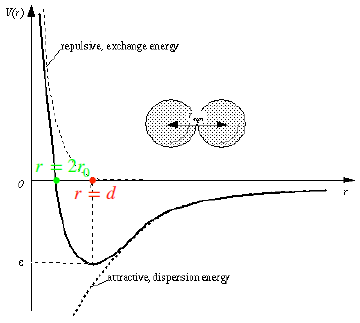
\includegraphics[width = 8cm]{van der Waals.png}
    \caption{Van der Waals potential. It is repulsive when $U(r) > 0$ (in the image indicated as $V(r)$}
    \label{fig:vanDerWaals}
\end{figure}

So we obtain: $ \frac{-J_2(\beta)}2 = b- \frac a{k_BT}$ and from the expression of the pressure:
$$ \boxed{p = k_BTn\left[1 + \left(b- \frac a{k_BT}\right)n\right]} + O(n^3)$$
and defining $n = N/V = 1/v$, we obtain the \textbf{van der Waals equation of a real gas}: 
$$ \boxed{\left(p - \frac a{v^2}\right)\left(v - b\right) = k_BT} $$

\vspace{30pt}

\gray{RECAP:
\boxed{\begin{tabular}{c c c}
     Microcanonical & Canonical & Grancanonical\\
     $\rho_{mc} = \frac 1{\omega(E)} \delta (\ham - E)$ & $\rho_c = \frac{e^{-\beta \ham}}{Z_N}$  & $\rho_{gc} = \frac {e^{-\beta(\ham - \mu N)}}\Z$ \\
     \\\\
     \multicolumn{3}{c}{$S = -k_B \angles{\log \rho} \stackrel{TD\ lim}= S_{Th} = k_B \log \underbrace{\sum(E)}_{\text{\#states}}$}
\end{tabular}}
}

\section{State counting and Entropy}
We have seen that the Boltzmann's universal law give a value for the entropy which (in the thermodynamic limit) is the same of the thermodynamic entropy. We also know from the variational principle of thermodynamics that the equilibrium corresponds to maximum entropy.

In this brief discussion, we fix our attention to the canonical ensemble, but similar considerations hold for the grancanonical one.

In some case, the energy is discretized and we use $E$ (instead of $\ham$) to indicate the energy level. Also, each energy level can be degenerate, meaning that more than one state have that energy. We indicate the degeneracy with $g_i = g(E_i)$.

We define the Boltzmann's weight as the probability to have energy $E$:
\begin{equation} \label{eq:boltzmann-weight}
\rho_E = \frac{e^{-\beta E}}{Z_N} \quad Z_N = \sum_E g_E e^{-\beta E} \implies S = -k_B\sum_E \rho_E \log \rho_E    
\end{equation}

\gray{In some cases, we can measure the energy of a system, but we can't look for its microstate. However this is a general formula and we can use it even when we don't know the microstate.}

Let’s look back at the ensemble description:
\begin{itemize}
    \item We have a very large number N of copies of the system, all described by the same values of macroscopic variables (macrostate), but corresponding to different values of microscopic variables (microstate)
    \item the probability that a given microstate occurs is the N-infinity limit of the frequency with which it appears (objective interpretation)
    \item all physics can be derived from knowing such probability distribution
\end{itemize}

Is there a principle to derive the probability distribution describing equilibrium?

\textbf{The probability distribution describing equilibrium is the one corresponding to maximum entropy, given the macroscopic constraints}.\\

\gray{Remark. This set-up (Boltzmann, Gibbs) is grounded on the idea that\\
i)  we have a clear identification of what a micro/macrostate is\\
ii) probability are defined a-priori quantities.
}

\begin{quote}
    Previously, one constructed a theory based on the equations of motion, supplemented by additional hypotheses of ergodicity, metric transitivity, or equal a priori probabilities, and the identification of entropy was made only at the end, by comparison of the resulting equations with the laws of phenomenological thermodynamics. Now, however, we can take entropy as our starting concept, and the fact that a probability distribution maximizes the entropy subject to certain constraints becomes the essential fact which justifies use of that distribution for inference.\\
    \gray{\textit{E.T Jaynes, Information theory and Statistical Mechanics, Phys. Rev. 106 (1957) 620}}
\end{quote}

\underline{\textbf{Inference problem}}
\begin{quote}
    The "objective" school of thoughts regards the probability of an event as an objective property of that event, always capable in principle of empirical measurement by observation of frequency ratios in a random experiment.\\
    On the other hand, the "subjective" school of thought regards probabilities as expressions of human ignorance; the probability of an event is merely formal expression of our expectation that the event will or did occur, based on whatever information is available.
\end{quote}

The inference problem is the following:\\
If the only info we have is that a certain function of $x$ has a given mean value $\angles f = \sum_{j=1}^N p_j f(x_j)$, what is the expectation value of another function $g(x)$?
We must use the probability distribution which has a maximum entropy subject to the constraints:
$$ \sum_{j=1}^N p_j = 1 \qquad \sum_{j=1}^N p_jf(x_j) = \angles {f(x)}$$
which is obtained by maximizing (Lagrange multipliers) the function:
$$ A = -\sum_{j=1}^N p_j\log p_j + \alpha \left(\sum_{j=1}^N p_j - 1 \right) + \gamma \left(\sum_{j=1}^N p_j(x_j) - \angles f \right)$$

\gray{Remark: It can be easily generalized to more observables and/or higher moments of the distribution}

\subsection{Probability distribution from maximum entropy principle}
We have a finite set of energy levels $E_r$, each with degeneracy $g_r$, on which we distribute a number $n_r$ of ensembles with total energy $E$ to distribute among $N$ copies of the system.
The number of ways to do that is $W_{\{n_r\}} = W^{(1)}_{\{n_r\}} W^{(2)}_{\{n_r\}}$.\\
where $W^{(1)}$ does not consider degeneracy so it counts how many ways we can put $n_r$ with $E_r$; while $W^{(2)}$ : the $n_r$ particles can be distributed in $g_r$ state.\\

We first consider classical particles, so they are distinguishable if they have different energy. So:
$$ W^{(1)}_{\{n_r\}} = \frac{N!}{n_1!n_2!\dots n_p!} \qquad\qquad \text{$N$ fixed} \quad n_1 \quad n_2 \quad \dots \quad n_r \quad \dots \quad n_p $$
$$W^{(1)}_{\{n_r\}} = \prod_r g_r^{n_r} \qquad\qquad \text{$E_r$ fixed} \quad \underbrace{\text{--- \quad --- \quad --- \quad --- \quad --- \quad}}_{n_r} g_r$$

From the maximum entropy principle, the equilibrium distribution corresponds to max entropy $ S = \log W_{\{n_r\}}$\\
with the constraints 
$$ N = \sum_r n_r \qquad E = \sum_r n_r E_r$$

So, in the classical case: 
$$W_{\{n_r\}} = N! \prod_{r=1}^p \frac{g_r^{n_r}}{n_r!} \qquad S = k_B \log W_{\{n_r\}}$$
\begin{align*}
    A &= k_B \log W_{\{n_r\}} + \alpha \left(N - \sum_r n_r\right) + \beta \left(E - \sum_r n_rE_r\right) \\
    &= k_B \left[\log N! + \sum_r \log g_r^{n_r} - \sum_r \log n_r!\right] + \alpha \left(N - \sum_r n_r\right) + \beta\left(E - \sum_r n_rE_r\right)\\
    &= k_B \left[N\log N \cancel{- N} + \sum_r n_r\log g_r - \sum_r \left(n_r\log n_r \cancel{-n_r}\right)\right] + \alpha \left(N - \sum_r n_r\right) + \beta\left(E - \sum_r n_rE_r\right)\\
    &= k_B \left[N\log N + \sum_r n_r\log g_r - \sum_r n_r\log n_r\right] + \alpha \left(N - \sum_r n_r\right) + \beta\left(E - \sum_r n_rE_r\right)
\end{align*}
To maximize this we derive:
$$ 0 = \left.\der A{n_r}\right|_{n_r = n_r^*} = \log g_r - \log n_r^* - 1 - \alpha - \beta E_r$$
and we find the number of particle that maximizes the entropy:
$$ \implies n_r^* = e^{-(1+\alpha)} g_r e^{-\beta E_r}$$
$$ N = \sum_r n_r^* = e^{-(1-\alpha)} \sum_r g_r e^{-\beta E_r}$$

And we can get the probability to get a particle in the energy level $r$:
$$ p_r = \frac{n_r^*}N = \frac{g_r e^{-\beta E_r}}{\sum_{r=1}^p g_r e^{-\beta E_r}} = \frac{g_r e^{-\beta E_r}}Z $$

So we get the same expression as in \ref{eq:boltzmann-weight}. Also, we obtain the Lagrange multiplier $\beta = \frac 1{k_BT}$\\

Quantum particle instead are always indistinguishable, not only when they have the same energy. Thus there is only one way to have $n_1$ particles with energy $E_1$, $n_2$ particles with energy $E_2$, etc... So: $W_{\{n_r\}}^{(1)} = 1$ and
$$ W_{\{n_r\}} = W^{(1)}_{\{n_r\}} W^{(2)}_{\{n_r\}} = W^{(2)}_{\{n_r\}}$$

For bosons, we can imagine of putting the particles in a line and draw boundaries to select in which energy level they are. So we have $n_r$ indistinguishable particles and $g_r-1$ indistinguishable boundaries. In total we have $n_r + g_r -1$ objects:
$$ W_{\{n_r\}} = W^{(2)}_{\{n_r\}} = \frac{(n_r+ g_r-1)!}{n_r!(g_r-1)!}$$

For fermions, we can put at most 1 particle for each "box", which is like saying that each box can be empty or with a ball ($n_r < g_r$). So it's like selecting $n_r$ objects out of $g_r$ possibilities:
$$W_{\{n_r\}} = W^{(2)}_{\{n_r\}} = \frac{g_r!}{n_r!(g_r-n_r)!}$$

\vspace{20pt}

We will derive again this distributions in the next chapter.